\documentclass{standalone}
\usepackage{pgfplots}
\pgfplotsset{compat=1.18}

\begin{document}

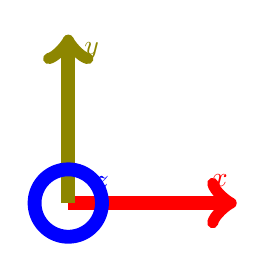
\begin{tikzpicture}
    \begin{axis}[
        axis lines=none,
        xlabel={$x$},
        ylabel={$y$},
        zlabel={$z$},
        xmin=-0.1, xmax=0.2,
        ymin=-0.1, ymax=0.2,
        zmin=-0.1, zmax=0.2,
        xtick=\empty,
        ytick=\empty,
        ztick=\empty,
        view={0}{90}, % View from the z-axis (top-down view)
        width=8cm,
        height=8cm,
        scale uniformly strategy=units only,
        every axis label/.style={font=\fontsize{40}{20}\selectfont}, % Increase font size
    ]
        % Draw arrows for the axes
        \addplot3[->, line width=5pt, red] coordinates {(0,0,0) (0.1,0,0)} node[pos=0.9, above]{$x$};
        \addplot3[->, line width=5pt, olive] coordinates {(0,0,0) (0,0.1,0)} node[pos=0.9, right]{$y$};
        \addplot3[line width=5pt,, blue, samples=100, domain=0:360] ({0.02*cos(x)}, {0.02*sin(x)}, 0) node[pos=0.5, above]{$z$};
    \end{axis}
\end{tikzpicture}

\end{document}